\chapter{فصل ‌جدید}‌\label{chap1}

%متن آزمایشی... ‌\\
%\section{بخش جدید}‌\\
%متن آزمایشی...‌\\
%\subsection{زیربخش جدید}‌\\
%متن آزمایشی...‌\\
%\subsubsection{زیرزیربخش جدید}‌\\
%متن آزمایشی...‌\\

%%%%%%%%%%%%%%%%%%%%%%%%%%%%%%%%%%%%%%

%\section{تولید پانویس}

%
%‌\\
%ما در این‌جا در لاتک%
%\LTRfootnote{LaTeX}
%یک پانویس%
%\footnote{پاورقی}
%تولید می‌کنیم. ما در این قسمت از
%\lr{LaTeX} 
%استفاده می‌کنیم.


%%%%%%%%%%%%%%%%%%%%%%%%%%%%%%%%%%%%%%

%\section{حروف‌چینی چندستونه}
%‌\\
%\begin{multicols}{2}
%	ی. متن آزمایشی. متن آزمایشی. متن آزمایشی. متن آزمایشی. متن آزمایشی. متن آزمایشی. متن آزمایشی. متن آزمایشی. متن آزمایشی. متن آزمایشی. متن آزمایشی. متن آزمایشی. متن آزمایشی. متن آزمایشی. متن آزمایشی. متن آزمایشی. متن آزمایشی. متن آزمایشی. متن آ
%\end{multicols}
%
%
%\begin{multicols}{3}
%	متن آزمایشی. متن آزمایشی. متن آزمایشی. متن آزمایشی. متن آزمایشی. متن آزمایشی. متن آزمایشی. متن آزمایشی. متن آزمایشی. متن آزمایشی. متن آزمایشی. متن آزمایشی. متن آزمایشی. متن آزمایشی. متن آزمایشی. متن آزمایشی. متن آزمایشی. متن آزمایشی. متن آزمایشی. متن آزمایشی. متن آزمایشی. 
%\end{multicols}

%%%%%%%%%%%%%%%%%%%%%%%%%%%%%%%%%%%%%%

%\section{حروف‌چینی فانتزی}
%‌\\
%\shapepar{\heartshape}
%متن آزمایشی. متن آزمایشی. متن آزمایشی.تن آزمایشی. متن آزمایشی. متن آزمایشی. متن آزمایشی. متن آزمایشی. متن آزمایشی. متن آزمایشی. متن آزمایشی. متن آزمایشی. متن آزمایشی. متن آزمایشی. متن آزمایشی.متن آزمایشی. متن آزمایشی. متن آزمایشی. متن متن آزمایشی. متن متن آزمایشی. متن متن آزمایشی. متن متن آزمایشی. متن متن آزمایشی. متن متن آزمایشی. متن متن آزمایشی. متن

%%%%%%%%%%%%%%%%%%%%%%%%%%%%%%%%%%%%%%

%\section{فهرست‌های درهم}
%‌\\


%\begin{itemize}
%	\item 
%	مهدی اخوان ثالث
%	\begin{itemize}
%		\item 
%		زمستان
%		\item
%		ارغوان
%		\begin{itemize}
%			\item 
%			به سبک شعر کهن
%		\end{itemize}
%	\end{itemize}
%\end{itemize}
%%%
%%%%%%%%%%%
%%
%\begin{enumerate}
%	\item 
%	مهدی اخوان ثالث
%	\begin{enumerate}
%		\item 
%		زمستان
%		\item
%		ارغوان
%		\begin{itemize}
%			\item 
%			به سبک شعر کهن
%		\end{itemize}
%	\end{enumerate}
%\end{enumerate}

%%%%%%%%%%%%%%%%%%%%%%%%%%%%%%%%%%%%%%

%\section{قضایا و...}
%‌\\

%\begin{theorem}
%فرض کنید تابع $f$ مشتق‌پذیر باشد...	
%\end{theorem}
%
%\begin{proof}
%	برای اثبات...	
%\end{proof}

%\begin{tcolorbox}
%متن آزمایشی...
%\end{tcolorbox}

%\begin{phbox}[breakable,label={myfreestyle}]{عنوان سوال}
%متن آزمایشی...
%\end{phbox}
%\begin{phboxr}[breakable,label={myfreestyle}]{عنوان سوال}
%
%	متن آزمایشی...%
%\footnote{آزمایشی}
%متن آزمایشی...%
%\LTRfootnote{Test}
%‌\\‌\\‌\\‌\\‌\\‌\\‌\\‌\\‌\\‌\\‌\\‌\\‌\\‌\\‌\\‌\\‌\\‌\\‌\\‌\\‌\\‌\\‌\\‌\\‌\\‌\\‌\\‌\\‌\\‌\\‌\\‌\\‌\\‌\\‌\\‌\\‌\\‌\\‌\\‌\\‌\\‌\\‌\\‌\\‌\\‌\\‌\\‌\\‌\\‌\\‌\\‌\\‌\\‌\\‌\\‌\\‌\\‌\\‌\\‌\\‌\\‌\\‌\\‌\\‌\\‌\\‌\\‌\\‌\\‌\\‌\\‌\\‌\\‌\\‌\\‌\\‌\\‌\\‌\\‌\\‌\\‌\\‌\\‌\\‌\\‌\\‌\\‌\\‌\\‌\\‌\\‌\\‌\\‌\\‌\\‌\\‌\\‌\\‌\\‌\\‌\\‌\\‌\\‌\\‌\\‌\\‌\\‌\\
%متن آزمایشی...
%\end{phboxr}

%%%%%%%%%%%%%%%%%%%%%%%%%%%%%%%%%%%%%%

%\section{ایجاد فضای خالی در متن} 

%‌\\
%به پایان آمد این دفتر حکایت همچنان باقی
%\hspace{1.5cm}
%به صد دفتر نشاید گفت حسب الحال مشتاقی
%\vspace{4cm}
%\noindent
%نه حسنت آخری دارد نه سعدی را سخن پایان
%\hspace{1.5cm}
%بمیرد تشنه مستسقی و دریا همچنان باقی
%‌\\
%\subsection{هم‌ترازی متن}
%‌\\
%\begin{flushleft}
%هم‌ترازی "متن" از سمت چپ
%\end{flushleft}
%\begin{flushright}
%هم‌ترازی "متن" از سمت راست
%\end{flushright}
%
%
%
%\begin{center}
%وسط‌چین‌کردن متن
%\end{center}
%\centerline{وسط‌چین‌کردن متن (2)}
%\centering
%وسط‌چین‌کردن متن (3)

%%%%%%%%%%%%%%%%%%%%%%%%%%%%%%%%%%%%%%
%
%\section{قلم}
%‌\\
%{\tiny
%متن مورد نظر...}
%{\scriptsize
%	متن مورد نظر...}
%{\footnotesize
%	متن مورد نظر...}
%{\small
%متن مورد نظر...}
%{\normalsize
%متن مورد نظر...}
%{\large
%متن مورد نظر...}
%{\Large
%متن مورد نظر...}
%{\LARGE
%متن مورد نظر...}
%{\huge
%متن مورد نظر...}
%{\Huge
%\textbf{متن مور}د نظر...}
%‌\\
%‌\\
%%%%%%
%{\Huge
%متن مورد نظر...}
%\normalsize
%متن مورد نظر...

%%%%%%%%%%%%%%%%%%%%%%%%%%%%%%%%%%%%%

%\section{قلم}
%‌\\
%\textrm{متن معمولی}\\
%\textbf{متن پررنگ}\\
%\textit{متن ایتالیک (خوابیده)}\\
%\underline{متن زیرخط‌دار}\\
%\fbox{متن داخل جعبه}\\
%\emph{متن تأکیدشده}\\
%‌\\
%‌\\
%\textit{
%	متن ایتالیک (
%	\emph{خوابیده}
%	)
%}\\

%%%%%%%%%%%%%%%%%%%%%%%%%%%%%%%%%%%%%%

%\section{تنظیم اندازه، نوع و رنگ قلم (فونت)}
%‌\\
%
%\defpersianfont\nast{IranNastaliq}  \defpersianfont\nastf[Scale=5]{IranNastaliq} 
%\defpersianfont\rednast[Color=red, Scale=3]{IranNastaliq}
%\nast{متن مورد نظر...} 
%\nastf{متن مورد نظر...} 
%\rednast{متن مورد نظر...} 
%\textcolor{blue}{این یک متن آزمایشی آبی است.}
%\textcolor{blue!50}{این یک متن آزمایشی آبی است.}

%%%%%%%%%%%%%%%%%%%%%%%%%%%%%%%%%%%%%%

\section{تصویر}
‌\\





%\begin{figure}[H] \label{Picture1}
%	\centering
%	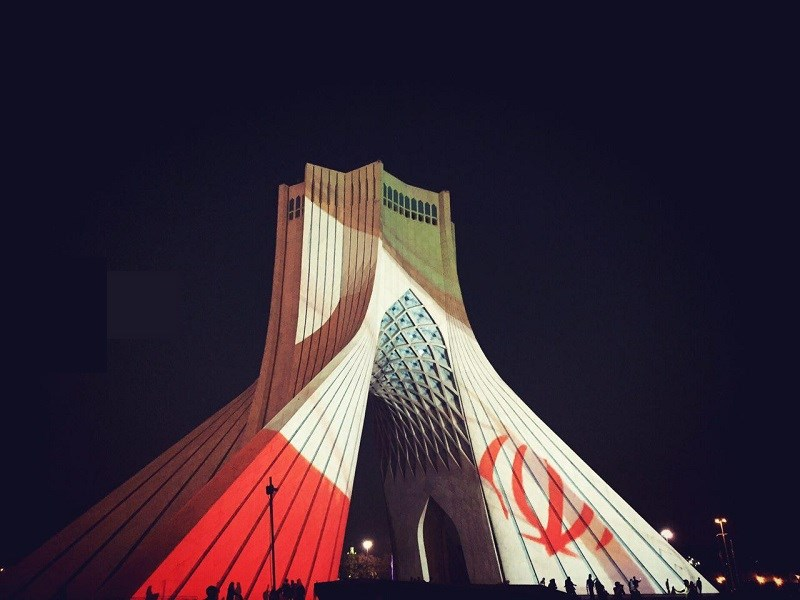
\includegraphics[width=5cm]{Picture1.png}
%	\caption{
%		تصویری از میدان آزادی
%	} 
%\end{figure}
%%%%%%%%%%%%%
%\begin{figure}[H] 
%	\centering
%	\includegraphics[height=5cm, width=5cm, angle=30]
%	{Picture1.png}
%	\caption{
%		تصویری از میدان آزادی
%	} \label{Picture1}
%\end{figure}
%%%%%%%%%%%%%
%\begin{figure}[H]  \centering
%	\subfigure[تصویر اول ]{ 		
%		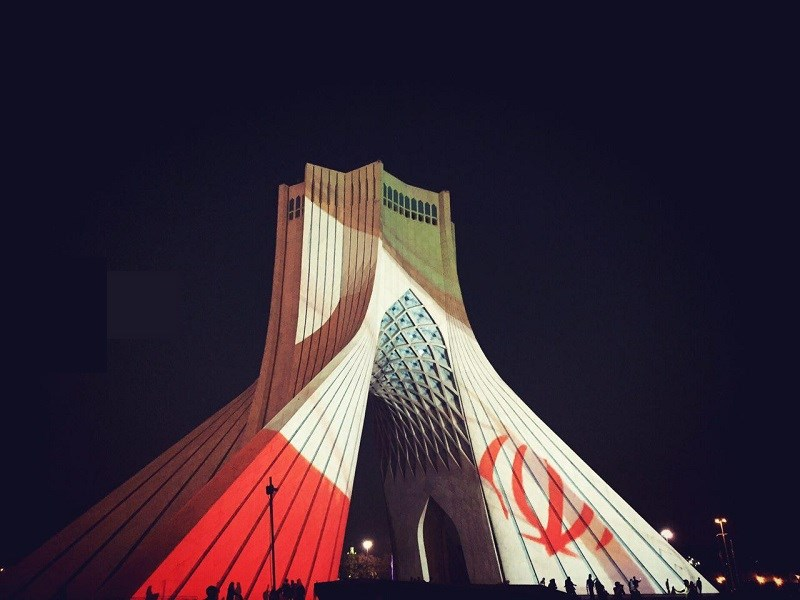
\includegraphics[width=5cm]{Picture1.png} \label{Picture1}}
%	\hspace{20mm}
%	\subfigure[تصویر دوم ]{ 	
%		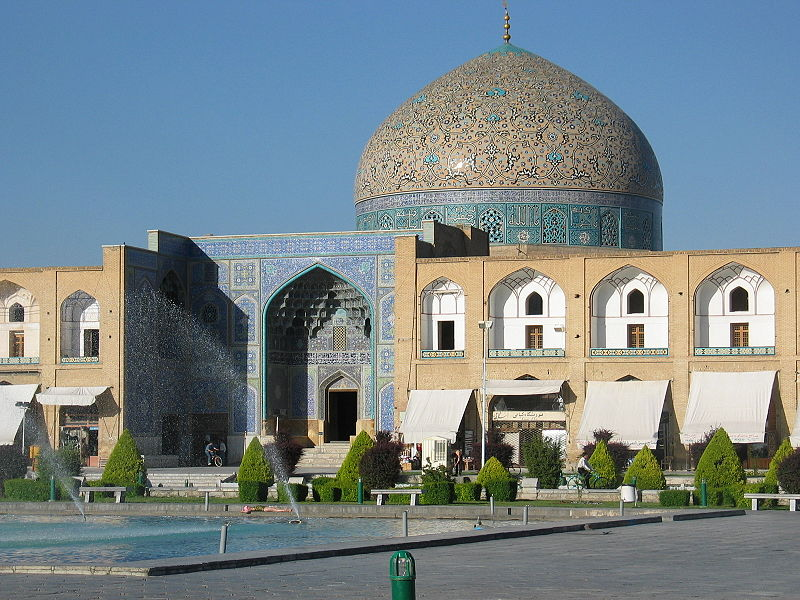
\includegraphics[width=5cm]{Picture2.png} \label{Picture2}}
%	\subfigure[تصویر سوم ]{
%		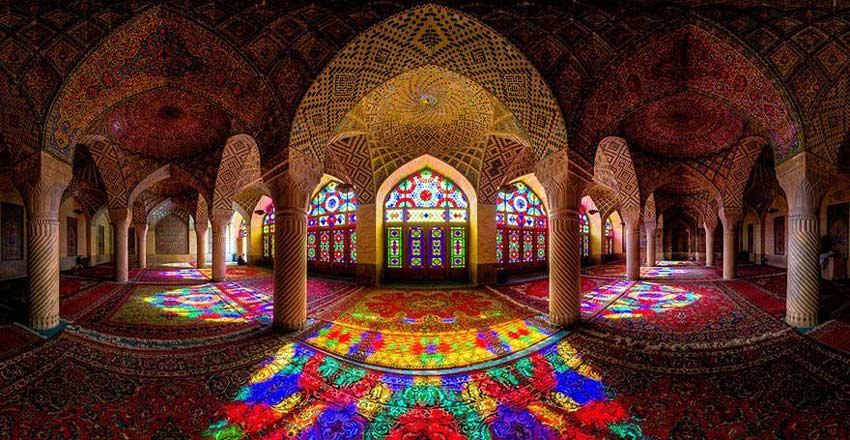
\includegraphics[width=5cm]{Picture3.png} \label{Picture1}}
%	\hspace{20mm}
%	\subfigure[تصویر چهارم]{
%		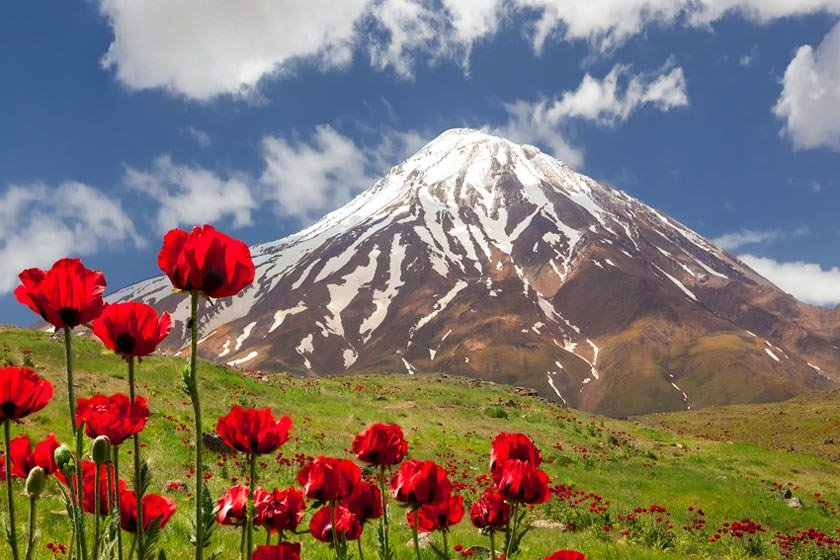
\includegraphics[width=5cm]{Picture4.png} \label{Picture2}}
%	\caption{
%		\subref{Picture1} میدان آزادی، 
%		\subref{Picture2} مسجد شیخ لطف‌الله،
%		\subref{Picture1} مسجد نصیرالملک، 
%		\subref{Picture2} کوه دماوند}\label{Pictures}
%\end{figure}

%%%%%%%%%%%%%%%%%%%%%%%%%%%%%%%%%%%%%%

%\section{جدول}
%‌\\
%\begin{table}[H]
%	\begin{center}
%		\begin{tabular}[H]{|c|c|p{4cm}|c||}
%			\hline
%			خانه11 & خانه12 &خانه13&خانه14\\
%			\hline	
%			\hline
%			\multicolumn{2}{|c|}{ادغام خانه21 و خانه22} & خانه23 & خانه24\\
%			\cline{2-3}
%			خانه31 & خانه32 &خانه33&خانه34\\
%			\hline		
%			خانه41 & خانه42 &خانه43&خانه44\\
%			\hline	
%		\end{tabular}
%	\end{center} 
%	\caption{کپشن جدول شماره‌ی یک}\label{Table1}
%\end{table}
%%%%%%%%%%%%
%% \usepackage{multirow}
%\begin{table}[]
%	\begin{center}
%		\begin{tabular}{|c|c|c|}
%			\hline
%			نشان متغیر & توضیح                            & واحد              \\ \hline
%			$F_T$      & \multicolumn{2}{c|}{\multirow{2}{*}{نیروی کشش قطار}} \\ \cline{1-1}
%			$F_D$      & \multicolumn{2}{c|}{}                                \\ \hline
%			$x$        & جابجایی قطار از مبدأ             & $m$               \\ \hline
%			$v$        & سرعت قطار                        & $m/s$             \\ \hline
%		\end{tabular}
%	\end{center} 
%\end{table}

%%%%%%%%%%%%%%%%%%%%%%%%%%%%%%%%%%%%%%
%
%\section{فرمول‌نویسی}
%‌\\
%\begin{equation}
%\left(\begin{array}{l}
%Q_{1} \\
%Q_{2}
%\end{array}\right) \equiv\left(\begin{array}{ll}
%C_{11} & C_{12} \\
%C_{21} & C_{22}
%\end{array}\right)\left(\begin{array}{l}
%V_{1} \\
%V_{2}
%\end{array}\right)
%\end{equation}
%جواب نهایی به‌صورت معادله‌ی 
%$x+1=0$ 
%خواهد بود.
%‌\\
%%%%%%%%%%%%%%%%%%%%%%
%\usepackage{amsmath}


%\begin{equation}\label{www}
%\lim_{x \to 1}
%\end{equation}


%\begin{equation} \label{eq1}
%x^{i+1} \times \sqrt[3]{y-2},\quad x_{i+1} = \frac{n+1}{n}, \quad \binom{n}{m}=\frac{n!}{m!(n-m)!}, \quad \boldsymbol{\varphi}, \quad \phi \varphi \epsilon \varepsilon, \qquad \mathbf{x}=(x_1,x_2,x_3)
%\end{equation}
%\begin{equation} \label{eq2}
%\sqrt{\frac1k \log_b x} = \sqrt{\tfrac1k \log_b x}
%\end{equation}
%\begin{equation}
%\bar{x}yz
%\left(\frac{x}{\text{متن}}\right)
%\end{equation}
%	%%%%%%%%%%%%%%%%%%%%%
%\begin{equation}
%\begin{bmatrix}
%1&2&3\\
%4&5&6\\
%7&8&9
%\end{bmatrix} 
%\end{equation}
%%%%%%%%%%%%%%%%%%%%%%
%\begin{equation}
%\begin{bmatrix}
%	
%	1 & 0 & \cdots & 0\\
%	
%	1 & 0 & \cdots & 0\\
%	
%	\vdots & \vdots & \ddots & \vdots \\
%	
%	1 & 0 & 0 & 0
%	
%\end{bmatrix}
%\end{equation}
%%%%%%%%%%%%%%%%%%%%%%
%\begin{equation}
%\left[\begin{array}{ll}
%1 & 0 \\
%1 & 0
%\end{array}\right]
%\end{equation}


%%%%%%%%%%%%%%%%%%%%%%%%%%%%%%%%%%%%%%

%\section{ارجاع‌دادن‌}\label{sec1.1}
%\subsection{ارجاع1}\label{subsec1.1}
%\subsubsection{ارجاع2}\label{subsubsec1.1}
%
%‌\\
%در
%\autoref{chap1}
%مشاهده می‌کنید. در
%\autoref{sec1.1}
%مشاهده می‌کنید. در
%\autoref{subsec1.1}
%مشاهده می‌کنید. در
%\autoref{subsubsec1.1}
%مشاهده می‌کنید. در قسمت
%\ref{sec1.1}
%مشاهده می‌کنید. در
%\nameref{sec1.1}
%مشاهده می‌کنید.
%در
%\autoref{Picture1}
%مشاهده می‌کنید.
%در
%\autoref{Picture1}
%مشاهده می‌کنید. در 
%\autoref{Table1}
%مشاهده می‌کنید. در 
%\autoref{eq1}
%مشاهده می‌کنید.
%\begin{figure}[H]
%	\centering
%	\includegraphics[height=5cm, width=5cm, angle=30]
%	{Picture1.png}
%	\caption{
%		تصویری از میدان آزادی
%	} \label{Picture1}
%\end{figure}
%
%\begin{table}[H]
%	\begin{center}
%		\begin{tabular}[H]{|c|c|p{4cm}|c||}
%			\hline
%			خانه11 & خانه12 &خانه13&خانه14\\
%			\hline	
%			\hline
%			\multicolumn{2}{|c|}{ادغام خانه21 و خانه22} & خانه23 & خانه24\\
%			\cline{2-3}
%			خانه31 & خانه32 &خانه33&خانه34\\
%			\hline		
%			خانه41 & خانه42 &خانه43&خانه44\\
%			\hline	
%		\end{tabular}
%	\end{center} 
%	\caption{کپشن جدول شماره‌ی یک}\label{Table1}
%\end{table}
%
%%\usepackage{amsmath}
%
%\begin{equation} \label{eq1}
%x^{i+1} \times \sqrt[3]{y-2},\quad x_{i+1} = \tfrac12\frac{n+1}{n}, \quad \binom{n}{m}=\frac{n!}{m!(n-m)!}, \quad \boldsymbol{\varphi}, \quad \phi \varphi \epsilon \varepsilon, \qquad \mathbf{x}=(x_1,x_2,x_3)
%\end{equation}
%
%
%
%برای مطالعه‌ی ادامه‌ی قضایا به 
%\cite{bidabad2007classification}
%مراجعه فرمایید \cite{aa}.
%









